% Define block styles
\tikzstyle{block} = [draw, rectangle, text centered, text width=6em, minimum height=5em, rounded corners=true, fill=white, fill opacity=0.9]
\tikzstyle{blockEmpty} = [rectangle, text centered, minimum height=1em, rounded corners=true, fill=white]
\tikzstyle{arrowtext} = [text width=4em, text centered]
\tikzstyle{arrow} = [draw, -latex]
\usetikzlibrary{shapes,backgrounds,calc}

\definecolor{red1}{RGB}{160,0,0}
\definecolor{green1}{RGB}{0,160,0}
\definecolor{blue1}{RGB}{0,0,160}

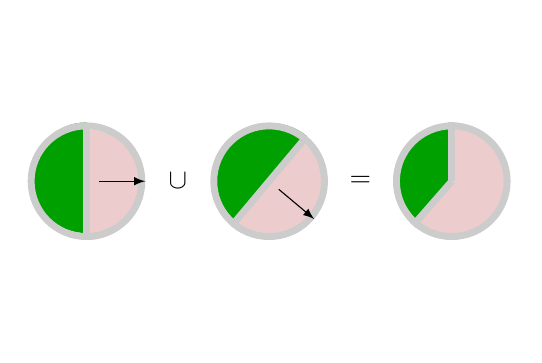
\begin{tikzpicture}[node distance=3.3em, auto]
  	% circle left
  	\node[shape=circle split,draw=gray!40,line width=0.25em,minimum size=4em, rotate=270] (circle2) {};
	\begin{scope}[on background layer]
    	\fill[red1!20, rotate=270] (circle2.base) (circle2.east) arc (0:180:2em)--cycle;
	    \fill[green1, rotate=270] (circle2.base) (circle2.west) arc (180:360:2em)--cycle;  
	\end{scope}
	\draw [arrow] (circle2.base) to (circle2.north);

	% +
	\node[right of=circle2] (plus) {$\cup$};

	% circle right
  	\node[right of=plus, shape=circle split,draw=gray!40,line width=0.25em,minimum size=4em, rotate=230] (circle1) {};
	\begin{scope}[on background layer]
    	\fill[red1!20, rotate=230] (circle1.base) (circle1.east) arc (0:180:2em)--cycle;
	    \fill[green1, rotate=230] (circle1.base) (circle1.west) arc (180:360:2em)--cycle;  
	\end{scope}
	\draw [arrow] (circle1.base) to (circle1.north);

	% =
	\node[right of=circle1] (equal) {=};

	% result
  	\node[right of=equal, shape=circle,draw=gray!40,line width=0.25em,minimum size=4em] (circle3) {};
	\draw[shape=line,draw=gray!40,line width=0.25em] (circle3.base) -- (circle3.north);
	\draw[shape=line,draw=gray!40,line width=0.25em] (circle3.base) -- ++(-1.4em, -1.6em);
	\begin{scope}[on background layer]
	    \fill[green1] (circle3.base) (circle3.north) ++(0.0em, -0.2em) arc (90:270:2em)--cycle;  
    	\fill[red1!20] (circle3.base) (circle3.south) ++(-1.3em, 0.5em) arc (-130:50:2em)--cycle;
	    \fill[red1!20, rotate=270] (circle3.base) (circle3.north) arc (180:0:2em)--cycle;  
	\end{scope}

    % Height of graphic should be 3cm, so it aligns with other subfigure
  	\node[right of=equal, rectangle, text centered, text width=0cm, minimum height=3.9cm, fill=white, node distance=0.3cm] (heightestimator) {};
\end{tikzpicture}
